\section{Construcción de los modelos}

    \subsection{Feature Engineering}
    \subsubsection{Chetocidad}
    
    Viendo las columnas presentes en \emph{dataset}, nos llamaron la atención varias características, que, cuando presentes en un inmueble, normalmente uno asociaría con un alto precio. Deseamos capturar esta relación haciendo uso de la técnica de \fe. Naturalmente, decidimos llamar a esta feature \textbf{chetocidad}. La definimos de la siguiente manera para cada \emph{entry}:

        $$chetocidad = gimnasio + piscina + usosmultiple + garages.$$
    
    Haremos uso de ella para segmentar el conjunto de datos, y poder predecir mejor el precio en cada uno.

    \begin{figure}[H]
        \centering
        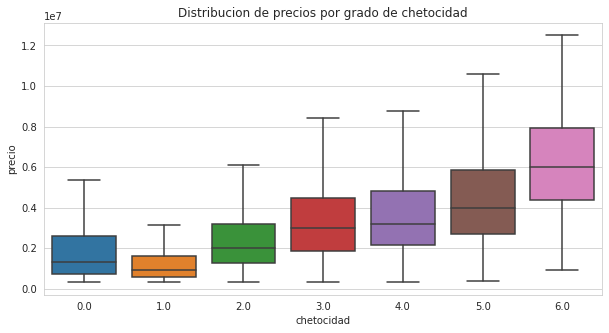
\includegraphics[scale=0.7]{img/cmp/precio/dist-chetocidad.png}
        \caption{}
        \label{fig:precio-dist-chetocidad}
    \end{figure}
    
    En la figura (\ref{fig:precio-dist-chetocidad}) se puede ver como a medida que el \emph{grado} de chetocidad incrementa, también lo hacen los precios.
    
    \subsubsection{WordCloud}
    
    Dos características interesantes presentes en el conjunto de datos son el \textbf{título} y la \textbf{descripción}. La intuición que tenemos es que, para inmuebles donde se parezcan estas dos, podrían llegar a tener características similares, por ejemplo el precio. Explicaremos nuestro procedimiento para el título, ya que para la descripción es un proceso análogo.
    
    Buscamos asignarle a cada inmueble un \emph{score} calculado a partir de su titulo. Para ello, la forma más simple que se nos ocurrió comienza con tomar todos los títulos de todos los inmuebles, y ver la cantidad de ocurrencias que tiene cada palabra del vocabulario que elijamos.
    
    Por ejemplo, si tuviéramos 3 propiedades, con títulos:
    
    \begin{verbatim}
        inmueble    titulo
        1           casa en venta
        2           casa en venta
        3           casa en venta en tijuana
    \end{verbatim}

    Omitiendo palabras como conectores ya que no aportan a lo que buscamos, nos quedarían las siguientes apariciones para cada palabra:
    
    \begin{verbatim}
        word        #
        casa        3
        venta       3
        tijuana     1
    \end{verbatim}
    
    Finalmente, para computar los \emph{scores} de cada titulo, tomamos el promedio de las apariciones de cada una de sus palabras. Esto nos da lo que llamamos \textit{frecuencia promedio de apariciones}, o, abreviado, \textit{avg\_freq\_title}:
    
    \begin{verbatim}
        inmueble    titulo                          avg_freq_title
        1           casa en venta                   (3 + 3) / 2 = 3
        2           casa en venta                   (3 + 3) / 2 = 3
        3           casa en tijuana                 (3 + 1) / 2 = 2
    \end{verbatim}
    
    De esta forma, logramos asignarle a cada inmueble un puntaje basado en su titulo.
    Nuestra hipótesis entonces es que resulta una característica sensata, que podría dar buenos resultados, pero tiene una fuerte dependencia en la naturaleza de los datos. Por su heterogeneidad, podría suceder que no necesariamente haya una relación entre inmuebles con títulos similares, a pesar de que sea intuitivo pensar que sí.
    
    \begin{figure}[H]
        \begin{subfigure}{.49\textwidth}
            \centering
            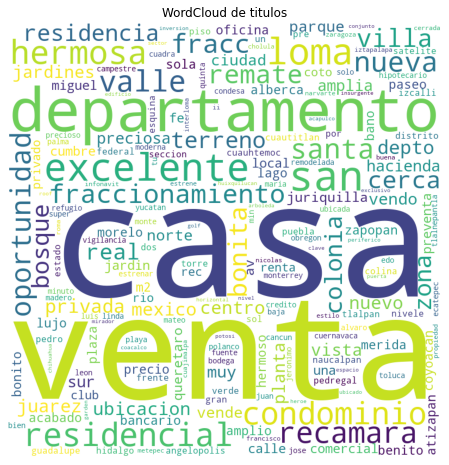
\includegraphics[scale=.5]{img/cmp/wc/wc-title.png}
            \caption{Títulos}
        \end{subfigure}
        \begin{subfigure}{.49\textwidth}
            \centering
            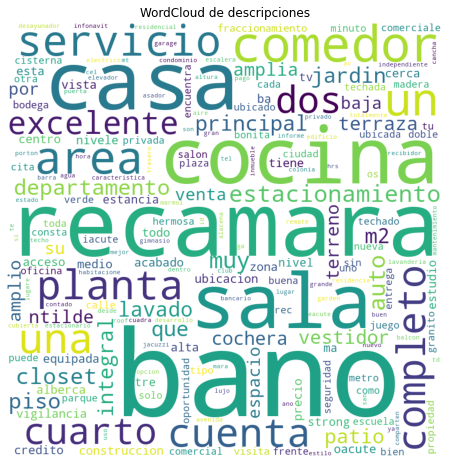
\includegraphics[scale=.5]{img/cmp/wc/wc-desc.png}
            \caption{Descripciones}
        \end{subfigure}
        \caption{WordClouds de campos de texto}
        \label{fig:wc}
    \end{figure}
    
    En la figura (\ref{fig:wc}), se puede observar como están distribuidas las distintas palabras que componen los campos de texto a considerar. Veamos las frecuencias obtenidas. 
    
    \begin{figure}[H]
        \centering
        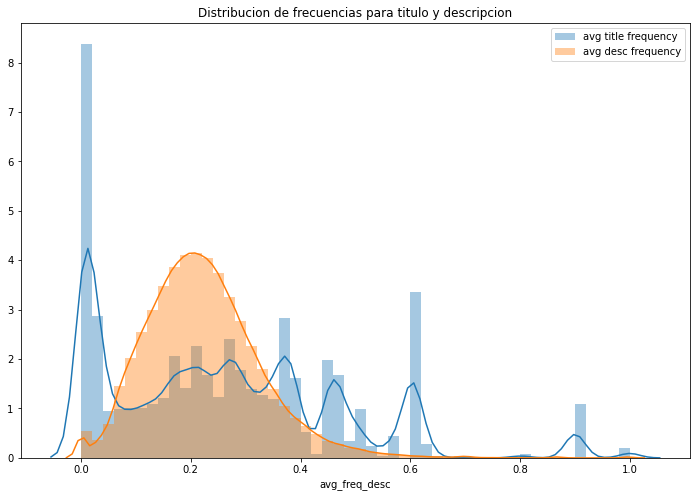
\includegraphics[scale=0.6]{img/cmp/wc/freq.png}
        \caption{Distribución de frecuencias}
        \label{fig:wc-freq}
    \end{figure}
    
    Y finalmente en (\ref{fig:wc-freq}) graficamos la distribución de los scores resultantes, que además normalizamos de 0 a 1 por min-max para simplificar.
    
    \subsection{Segmentación}
    
    Las variables categóricas que elegimos para segmentar el conjunto de datos son diferentes para cada variable a predecir, pero siempre incluimos la opción de \textbf{no} segmentar, para tenerla como base. 
    
    Para fortalecer nuestras intuiciones, graficamos en algunos casos a modo de ejemplo la distribución que tienen los datos segmentando por las variables a considerar. Que sean conjuntos que varían mucho entre sí, incluso disjuntos, nos llevaría a pensar que puede valer la pena entrenar a los clasificadores por separado.
    
    \subsubsection{Precio}
    
    Consideramos,
    
    \begin{itemize}
        \item \textbf{Provincia}: Es a la que le tenemos más expectativa. Como se puede ver en \ref{fig:precio-dist-provincia}, está bien marcada la diferencia entre las distribuciones de los precios para cada ciudad, y luego consideramos que verlas por separado evitará ruido, logrando que expliquemos mejor el precio.
        
            \begin{figure}[H]
                \centering
                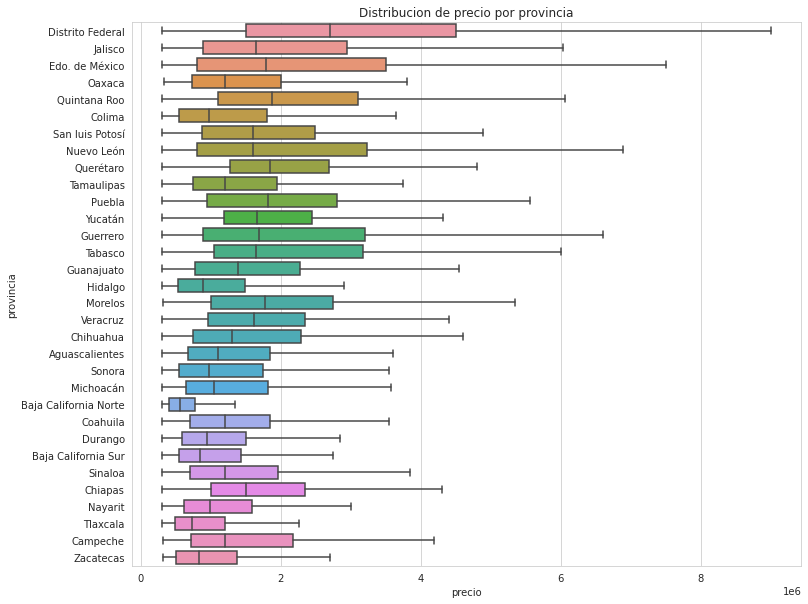
\includegraphics[scale=0.45]{img/cmp/precio/dist-provincia.png}
                \caption{Distribución por provincia}
                \label{fig:precio-dist-provincia}
            \end{figure}
        
        \item \textbf{Ciudad}: Diferentes ciudades tendrán diferentes situaciones económicas, y diferentes tipos de inmuebles con diferentes precios. Como son muchas (~800) podría llegar a generar un problema ya que los conjuntos de datos resultantes serán muy pequeños.
        \item \textbf{Chetocidad}: Como ya fue discutido en la figura \ref{fig:precio-dist-chetocidad}, inmuebles mas chetos tienden a ser mas caros.
        \item \textbf{Antiguedad}: Los inmuebles mas antiguos tienden a ser más caros.
    \end{itemize}
    
    \subsubsection{Metros cubiertos}
    
    Consideramos las siguientes,
    
    \begin{itemize}
        \item \textbf{Tipo de propiedad}: Intuitivamente, cada tipo de propiedad tendrá un cantidad de metros cubiertos que varíe. Nuestra hipótesis es que esta será la mejor.
        
        \begin{figure}[H]
            \centering
            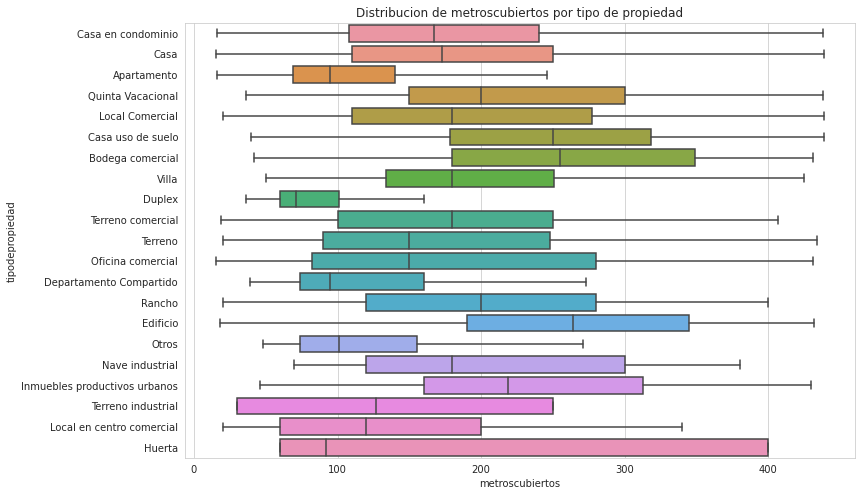
\includegraphics[scale=0.45]{img/cmp/metroscubiertos/dist-tipodepropiedad.png}
            \caption{Distribución por tipo de propiedad}
            \label{fig:m2-dist-prop}
        \end{figure}
        
        \item \textbf{Antiguedad}: Las casas más antiguas suelen ser más grandes, mientras que las más nuevas más chicas. Como se puede ver en \ref{fig:m2-dist-ant}, no es tan pronunciada como esperábamos.
        
        \begin{figure}[H]
            \centering
            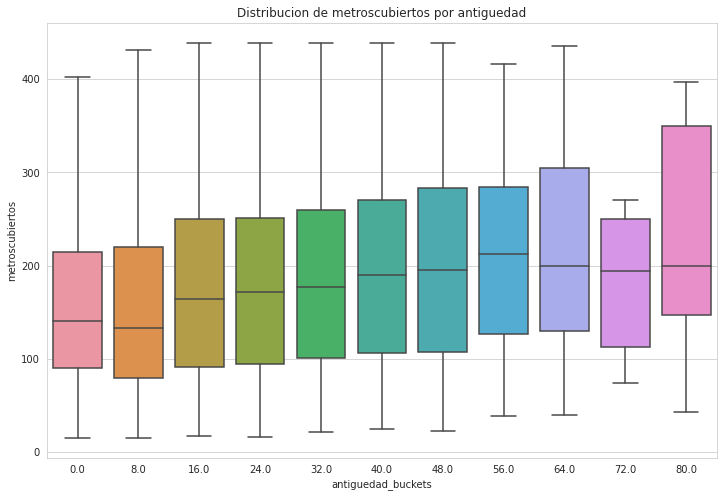
\includegraphics[scale=0.45]{img/cmp/metroscubiertos/dist-antiguedad.png}
            \caption{Distribución por antiguedad}
            \label{fig:m2-dist-ant}
        \end{figure}

        \item \textbf{Chetocidad}: A pesar de que este feature fue introducido originalmente para precios, las casas mas chetas suelen ser más grandes. Pero en la figura \ref{fig:m2-dist-chet} se observa como esta relación no es tan pronunciada como en el caso de la variable precio.
        
        \begin{figure}[H]
            \centering
            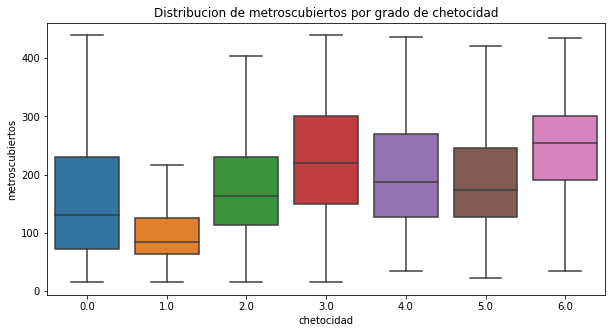
\includegraphics[scale=0.45]{img/cmp/metroscubiertos/dist-chetocidad.png}
            \caption{Distribución por chetocidad}
            \label{fig:m2-dist-chet}
        \end{figure}
    \end{itemize}
    
    \subsubsection{Segmentar o no segmentar, esa es la cuestión}
    
    Como discutimos anteriormente, al segmentar, un riesgo que corremos es que los conjuntos de datos resultantes sean demasiado pequeños, lo que llevaría a que el clasificador resultante esté potencialmente \textit{overfitteado} a esos datos. Por ejemplo, al haber tantas ciudades, es posible que esto suceda al segmentar por ellas.

    \subsection{Selección de features}
    
    Una vez definidas las categorías por las cuáles queríamos segmentar, necesitábamos alguna manera de determinar, qué features debía incluir finalmente nuestro modelo. Entonces, un primer paso era, basados en los resultados de la matriz de correlación (Figura \ref{corr}), filtrar los features mas útiles a considerar para la selección en el segundo paso. Este primer paso se puede observar a continuación:
    \begin{figure}[H]
        \centering
        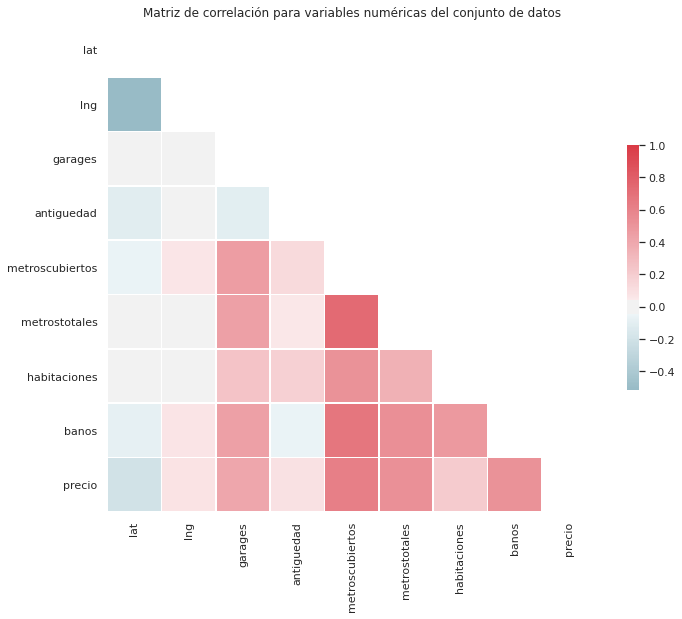
\includegraphics[scale=0.5]{img/cmp/1_corr.png}
        \caption{Matriz de correlación}
        \label{corr}
    \end{figure}
    
    Considerando solo las variables con un índice de correlación mayor a 0.2 con precio en esta matriz, obtuvimos el conjunto inicial de features compuesto por:
    

        \begin{verbatim}
            features = [
                    'metroscubiertos',
                    'antiguedad',
                    'banos',
                    'garages',
                    'metrostotales',
                    'habitaciones'
            ]
        \end{verbatim}
    
    Luego, el segundo paso consistió en utilizar el método \fss \ que se explicó en secciones anteriores, para seleccionar los features finales para cada modelo basándonos en los obtenidos en el paso 1. En este paso tuvimos en cuenta distintos tipos de modelos, entre ellos, regresores lineales, polinomiales y de proyección. Los resultados para distintas selecciones de features para cada modelo se observan en la figura (\ref{fss}):
     
    \begin{figure}[H]
        \centering
        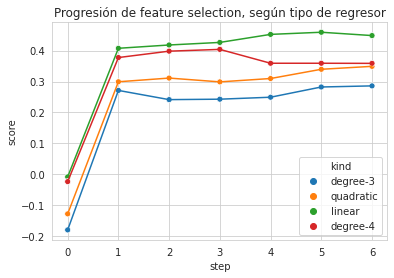
\includegraphics[scale=0.6]{img/cmp/1_fss.png}
        \caption{Progresión del score (que equivale a R2) para distintos modelos a medida que se sumaban variables a cada uno.}
        \label{fss}
    \end{figure}
    Consideramos que la mejor selección de features para cada modelo en en este caso era la que maximizaba el score.
    
    \subsection{Clasificadores a considerar}
    
    Los clasificadores que comparamos se muestran a continuación, donde cada uno se combino con cada posible segmentación descripta anteriormente. Para cada uno definimos un \textit{kind}, que podía ser polinomial o de proyección, y una lista de features a considerar, las cuales pueden haber sido escogidas por pura intuición o mediante un mecanismo automático como \fss.
    
    \paragraph{Precio}\mbox{}\vspace{1em}
    
    Incluimos como control el regresor más simple: explicar precio a través de metroscubiertos con una proyección.
    
    \begin{figure}[H]
    \centering
    \begin{tabular}{ |c|c|c| } 
    \hline
    kind                    & feature       & elección \\ \hline
    projection              & metroscubiertos & control \\ \hline
    projection con freqs    & metroscubiertos, avg\_freq\_title, avg\_freq\_desc & a ojo \\ \hline
    quadratic               & metroscubiertos, metrostotales & forward stepwise \\ \hline
    linear                  & metroscubiertos, metrostotales, banos, habitaciones & forward stepwise \\ \hline
    degree 4                & metroscubiertos, metrostotales, habitaciones & forward stepwise \\ \hline
    \end{tabular}
    \caption{Features por cada clasificador}
    \end{figure}
    
    \subsection{Metroscubiertos}
    
    Las features en este caso fueron elegidas a ojo, y las que consideramos que mejor podían explicar los metros cubiertos de un inmueble son las \textit{habitaciones}
    , \textit{cantidad de baños} y finalmente \textit{precio}. Los tipos a considerar son \textit{linear}, \textit{quadratic} y \textit{projection}.

\section{Discusión de los resultados}

A continuación procedemos a presentar los resultados obtenidos para cada clasificador. Consideramos las métricas de scoring \textit{r2}, \textit{rmse} y \textit{rmsle}. Y ordenamos los resultados por \textit{r2}.

\subsection{Precio}

\begin{figure}[H]
\centering
\begin{tabular}{ |c|c|c|c|c|c| } 
\hline
\textbf{rank} & kind & segment\_by & r2 & rmse & rmsle \\ \hline
0 & linear & provincia & 0.5419 & 1191109.9895 & 0.5043 \\ \hline
1 & linear & None & 0.4512 & 1307140.9522 & 0.5536 \\ \hline
2 & degree 4 & None & 0.4285 & 1431781.8520 & 0.5671 \\ \hline
3 & projection con freqs & antiguedad & 0.4191 & 1563665.8240 & 0.5833 \\ \hline
4 & projection & antiguedad & 0.4187 & 1564135.4745 & 0.5764 \\ \hline
5 & quadratic & None & 0.4137 & 1456341.1900 & 0.5747 \\ \hline
6 & projection con freqs & None & 0.4009 & 1600473.7443 & 0.5850 \\ \hline
7 & projection & None & 0.3941 & 1609558.2153 & 0.5928 \\ \hline
8 & degree 4 & chetocidad & 0.3921 & 1392346.0420 & 0.5670 \\ \hline
9 & degree 4 & provincia & 0.3892 & 1463775.4949 & 0.5861 \\ \hline
10 & linear & antiguedad & 0.3811 & 1374499.6945 & 0.5946 \\ \hline
11 & quadratic & provincia & 0.3624 & 1509252.7953 & 0.5697 \\ \hline
12 & projection con freqs & provincia & 0.3486 & 1662345.9426 & 0.5977 \\ \hline
13 & quadratic & chetocidad & 0.3466 & 1451725.5995 & 0.6199 \\ \hline
14 & linear & chetocidad & 0.3423 & 1444285.9409 & 0.6493 \\ \hline
15 & projection & provincia & 0.3420 & 1671243.2280 & 0.5878 \\ \hline
16 & projection & chetocidad & 0.3348 & 1572625.8697 & 0.6009 \\ \hline
17 & projection con freqs & chetocidad & 0.3269 & 1581599.8504 & 0.6171 \\ \hline
18 & linear & ciudad & 0.2782 & 1461909.1757 & 0.6008 \\ \hline
19 & quadratic & antiguedad & 0.2776 & 1601084.2432 & 0.5791 \\ \hline
20 & projection & ciudad & 0.2403 & 1776188.0175 & 0.6095 \\ \hline
21 & projection con freqs & ciudad & 0.1658 & 1853461.1484 & 0.6400 \\ \hline
22 & degree 4 & antiguedad & -0.9848 & 2516549.2875 & 0.5691 \\ \hline
23 & quadratic & ciudad & -4.1010 & 3718277.8536 & 0.6969 \\ \hline
24 & degree 4 & ciudad & -9267.9664 & 98474551.6608 & 0.6953 \\ \hline
\end{tabular}
\caption{Resultados de prediccion de precios por tipo y segmentación}
\label{table:results-precio}
\end{figure}

\begin{itemize}
    \item El mejor de todos fue el lineal, segmentando por provincia lo cual se condice con nuestras expectativas. Segmentar por provincia permite capturar las particularidades de cada zona geográfica, y realizar una regresión lineal sobre cada segmento nos permite abstraernos de la naturaleza exacta de los datos, simplemente trazando una recta, lo cual se generaliza mejor a la hora de predecir nuevos datos.
    
    \item El peor de todos, con rango 24, segmenta por ciudad con una regresión polinomial de grado 4. Esto causa que al haber tantas ciudades, como los segmentos son muy chicos, el polinomio de grado 4 se ajusta demasiado a los datos, produciendo así un overfitting que no predice para nada bien datos desconocidos.
    
    \item Como se puede ver en el rank 3, la feature derivada de las frecuencias promedio de las palabras del titulo y descripción lograron un resultado razonable, como era de esperarse.
    
    \item Algo que definitivamente no esperamos era que el hecho de \textbf{no} segmentar, que habíamos agregado meramente como control, resulte tan bueno. Esto en parte puede explicarse por la sanitización del conjunto de datos (i.e dropna) realizada antes de correr cada uno. Esto resultó en un conjunto de datos en algunos casos bastante más reducido, con lo que el impacto de segmentar era muchísimo menor.
    
    \item Otro resultado inesperado fue que regresores polinomiales de grados mayores no necesariamente eran mejores. A pesar de tener mas granularidad en los coeficientes, estos fueron especialmente propensos a sesgo de selección.

\end{itemize}

Veamos la distribución de los errores cometidos

\begin{figure}[H]
    \centering
    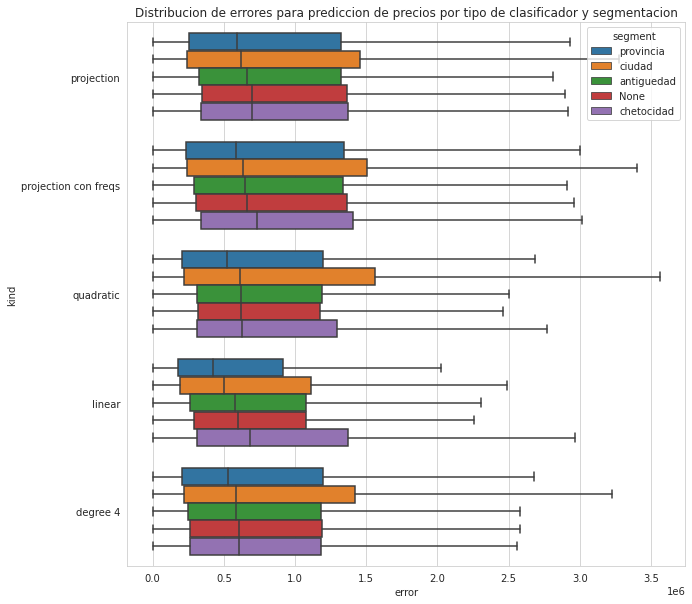
\includegraphics[scale=0.5]{img/cmp/precio/err-by-kind-seg.png}
    \caption{Distribución de errores absolutos cometidos para cada tipo de clasificador por segmento al predecir precio}
    \label{err-precio}
\end{figure}

En \ref{err-precio} se puede ver que ciudad fue el criterio de segmentación que más error tuvo, y curiosamente, si bien chetosidad fue de los mejores para casi todos, en linear fue el que más error tuvo.

\subsection{Metros cubiertos}

\begin{figure}[H]
\centering
\begin{tabular}{ |c|c|c|c|c|c| } 
\hline
\textbf{rank}    & kind    & segment\_by  & r2    & rmse    & rmsle \\ \hline
0   & projection  & tipodepropiedad   & 0.6980 & 51.9076  & 0.2914 \\ \hline
1   & linear  & tipodepropiedad   & 0.6949 & 52.1679  & 0.2967 \\ \hline
2   & quadratic    & tipodepropiedad    & 0.6949  & 52.1679   & 0.2967 \\ \hline
3   & linear  & None  & 0.6288    & 57.5751 & 0.3314 \\ \hline
4   & linear  & antiguedad    & 0.6284  & 57.6881   & 0.3353 \\ \hline
5   & quadratic    & antiguedad & 0.6284   & 57.6881    & 0.3353 \\ \hline
6   & projection  & antiguedad    & 0.6174  & 58.5364   & 0.3476 \\ \hline
7   & projection  & None  & 0.6166    & 58.5094 & 0.3492 \\ \hline
8   & linear  & chetocidad    & 0.5981  & 56.3890   & 0.3369 \\ \hline
9   & quadratic    & chetocidad & 0.5981   & 56.3890    & 0.3369 \\ \hline
10  & projection    & chetocidad   & 0.5832 & 57.4151  & 0.3383 \\ \hline
11  & quadratic  & None  & 0.4090    & 72.6409 & 0.4626 \\ \hline
\end{tabular}
\caption{Resultados por clasificador para la predicción de metros cubiertos}
\label{table:results-m2}
\end{figure}

Como se puede ver, nuestras intuiciones sobre el tipo de propiedad fueron acertadas, ya que los regresores que segmentaban por esta característica ocuparon los primeros puestos en el ranking. Además, los features elegidos fueron buenos, ya que se llegó a casi 0.7 de r2, lo cual indica que es un regresor cercano al ideal, o al menos mucho mas que para precio.

\begin{figure}[H]
    \centering
    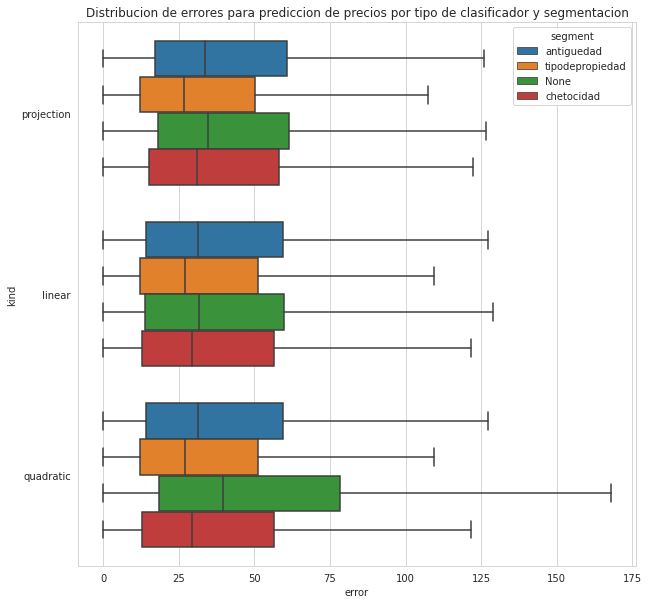
\includegraphics[scale=0.5]{img/cmp/metroscubiertos/err-por-kind-seg.png}
    \caption{Distribución de errores absolutos cometidos para cada tipo de clasificador por segmento al predecir metroscubiertos}
    \label{err-m2}
\end{figure}

En \ref{err-m2} se ve un gráfico del mismo estilo que para precio (fig. \ref{err-precio}). Afortunadamente, en este caso segmentar tendió a ser mejor que no hacerlo, y además, se puede ver como tipodepropiedad es el que menor error tuvo.